% --- SECCIÓ 4: METODOLOGIA ---
\apartat{Metodologia de Recerca}
El rigor científic d'aquest treball es fonamenta en una metodologia de tall qualitatiu i experimental, adaptada a la naturalesa humana i tecnològica del projecte.

% --- ESQUEMA DE FLUX DE METODOLOGIA ---
\begin{figure}[ht]
    \centering
    \begin{tikzpicture}[node distance=1cm, auto,
        metstep/.style={rectangle, draw, fill=RoyalBlue!10, text width=12cm, text centered, rounded corners, minimum height=2.5em, font=\small, drop shadow},
        arrow/.style={thick,->,>=stealth, RoyalBlue}]
        
        \node [metstep] (s1) {\textbf{Fase 1: Diagnòstic} \\ Identificació de barreres comunicatives.};
        \node [metstep, below=of s1] (s2) {\textbf{Fase 2: Validació Externa} \\ Entrevistes a professionals de la Fundació Horitzó.};
        \node [metstep, below=of s2] (s3) {\textbf{Fase 3: Disseny Tècnic} \\ Selecció d'estímuls i planificació ergonòmica.};
        \node [metstep, below=of s3] (s4) {\textbf{Fase 4: Realització Física} \\ Construcció del prototip funcional.};
        \node [metstep, below=of s4] (s5) {\textbf{Fase 5: Avaluació} \\ Recollida d'evidències d'ús.};
        
        \draw [arrow] (s1) -- (s2);
        \draw [arrow] (s2) -- (s3);
        \draw [arrow] (s3) -- (s4);
        \draw [arrow] (s4) -- (s5);
    \end{tikzpicture}
    \caption{Full de ruta metodològic del projecte.}
\end{figure}

\subsection{Disseny i Desenvolupament del Prototip}
\begin{enumerate}
    \item \textbf{Recerca de referents:} Anàlisi d'espais Snoezelen\footnote{Sales de relaxació i estimulació multisensorial.} per triar els colors i textures més efectius.
    \item \textbf{Selecció de materials:} Ús de components segurs (fustes polides, LEDs de 12V, textures naturals com suro i lli).
    \item \textbf{Verificació d'usabilitat:} Proves de pressió per assegurar que qualsevol usuari pot interactuar amb la taula sense esforç excessiu.
\end{enumerate}

\begin{figure}[ht]
    \centering
    \begin{tcolorbox}[colback=white, colframe=RoyalBlue!20, arc=5pt, boxrule=0.5pt, left=2pt, right=2pt, top=2pt, bottom=2pt, shadow={1pt}{-1pt}{0pt}{black!5}]
        \centering
        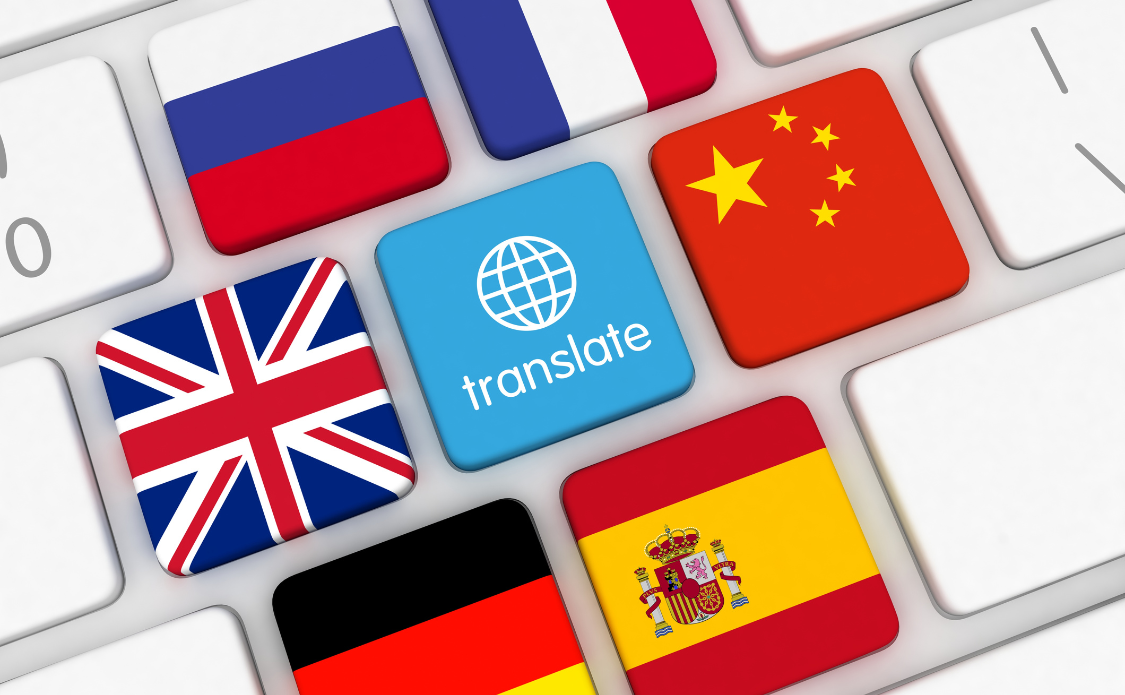
\includegraphics[width=0.8\textwidth]{imatges/Overcoming-Language-Barriers-Enhancing-Communication-Skills-in-a-Multicultural-Workplace-with-Hospitality-tecles_d'ordinador_amb-diferents_banderes_de_diferents_païssos_amb_el_botó_de_translate_al_mitg.png}
    \end{tcolorbox}
    \caption{La tecnologia com a pont universal per superar barreres comunicatives.}
\end{figure}
